\section{Vivado Report}

In this last section an \textbf{automatic synthesis} will be done, through the tool \textbf{Xilinx Vivado}. The target working device is the FPGA \textit{xc7z010clg400-1} and the three steps that will be analyzed are the following:

\begin{enumerate}
    \item \textbf{Elaborated Design} Analysis.
    \item \textbf{Synthesis} and Report analysis.
    \item \textbf{Implementation} and Report analysis.
\end{enumerate}

\subsection{Elaborated Design Analysis}

In this first part will be analyzed the \textbf{Elaborated Design}, that is the Vivado representation of the Linear Interpolator at the \textbf{Register Transfer Level}. It should be equal to the structure defined in the  Architecture Description Section.

\begin{figure}[H]
    \centering
    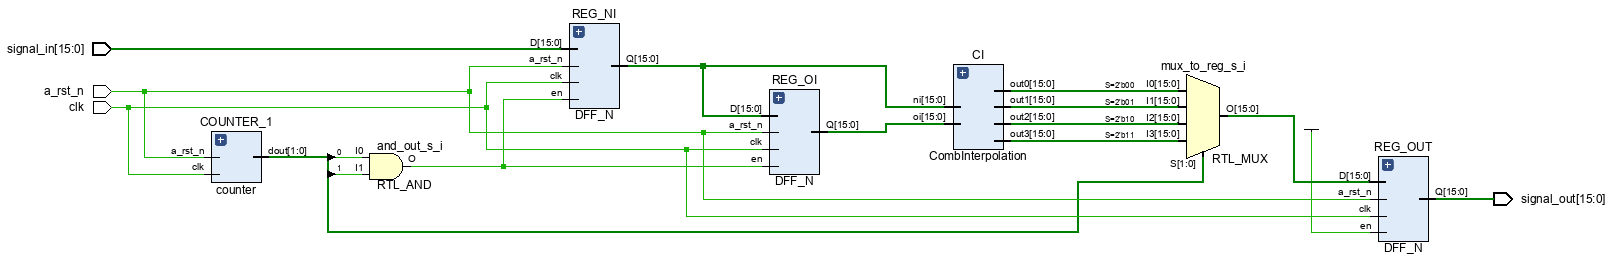
\includegraphics[width=1\textwidth]{img/Chapter5/Elaborated.png}
    \caption{Elaborated Design}
    \label{fig:ED}
\end{figure}

From the figure above is clear that the circuit respects the structure chosen in the planning stage, so it's possible to start the synthesis.

\subsection{Synthesis Analysis}

In this phase the Elaborated Design previously generated will be \textbf{translated} in circuits that the FPGA \textbf{can implement}. This will be done respecting all given \textbf{constraints}. In this case the only constraint is the clock, that must have a period of $8ns$.

The synthesis result is the following:

\begin{figure}[H]
    \centering
    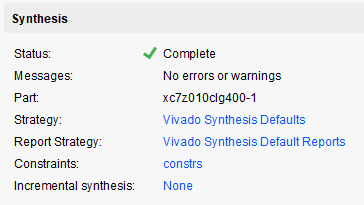
\includegraphics[width=0.5\textwidth]{img/Chapter5/SyntesisResult.png}
    \caption{Synthesis Result}
    \label{fig:SR}
\end{figure}

There are no errors or warnings, so it's possible to study the reports.

\subsubsection{Timing Report and Critical Path}

The \textbf{timings} obtained are as follows:

\begin{figure}[H]
    \centering
    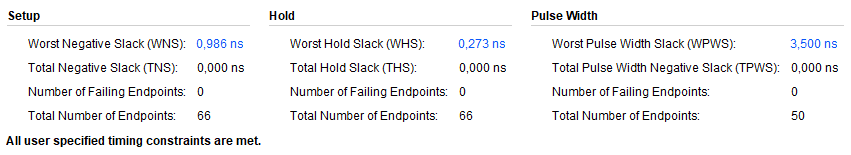
\includegraphics[width=1\textwidth]{img/Chapter5/SyntesisTiming.png}
    \caption{Timing Report}
    \label{fig:STR}
\end{figure}

First of all, there are \textbf{no negative slacks}, so the clock with a period of $8ns$ is clearly enough for the produced design. Moreover, the \textbf{worst negative slack} is $0.986ns$, so the clock can be at least faster of this value.

Analyzing the \textbf{synthesized design}, the \textbf{critical path} is the following:

\begin{figure}[H]
    \centering
    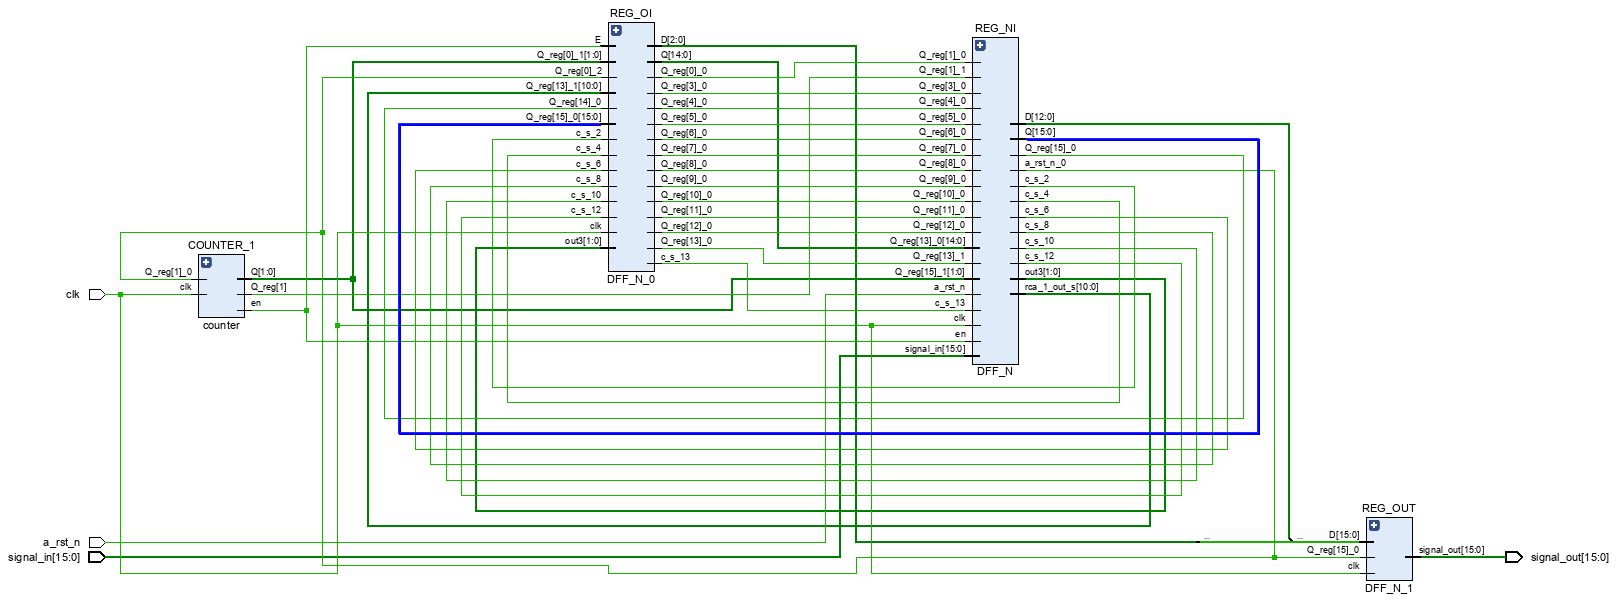
\includegraphics[width=1\textwidth]{img/Chapter5/SyntesisSetupCrit.png}
    \caption{Critical Path for Setup time}
    \label{fig:SCPS}
\end{figure}

\subsubsection{Utilization Analysis}

The \textbf{utilization report} obtained are as follows:

\begin{figure}[H]
    \centering
    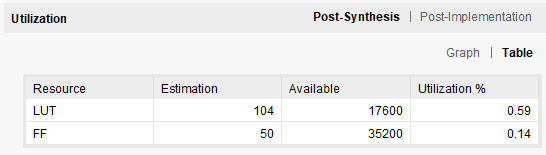
\includegraphics[width=0.6\textwidth]{img/Chapter5/SyntesisUtilization.png}
    \caption{Utilization Report}
    \label{fig:SU}
\end{figure}

The utilization for \textbf{Look Up Tables} and \textbf{Flip Flops} are lower then the $1\%$, so the FPGA has all resources needed to implement this circuit.

\subsubsection{Power Consumption Analysis}

The last report is about the \textbf{power consumption}. This is a very rough estimation, but allows to have a general idea of the circuit's power requirements.

\begin{figure}[H]
    \centering
    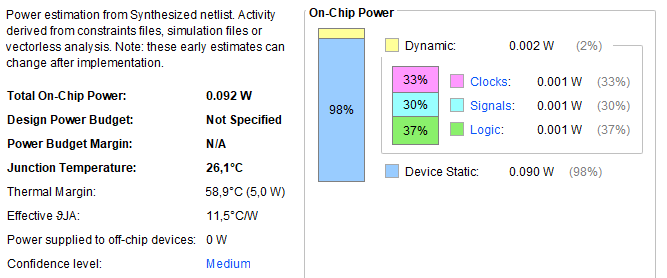
\includegraphics[width=1\textwidth]{img/Chapter5/SyntesisPower.png}
    \caption{Power Report}
    \label{fig:SPR}
\end{figure}

The \textbf{general consumption} is lower than  $100mW$. Moreover, it's clear that the percentage of static power is much greater than the dynamic power. So it's possible to say that the \textbf{switching activity} in this circuit is relatively low.

\subsection{Implementation analysis}

In this phase the \textbf{place and route} will be performed by Vivado, with some useful \textbf{optimizations}. In general this phase is preceded by the \textbf{I/O Planning}, in which the I/O Physical Ports of the FPGA are associated with the I/O Ports of the Elaborated Design. But the FPGA has not enough ports to implement an input and an output of 16 bit. So the implementation will be performed in \textit{Out of Context Mode}, that allows to do implementation without I/O Planning. 

The implementation result is the following:

\begin{figure}[H]
    \centering
    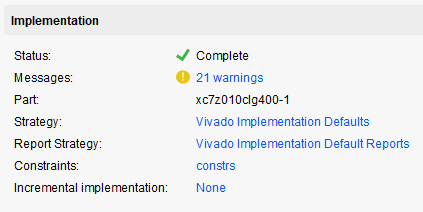
\includegraphics[width=0.5\textwidth]{img/Chapter5/ImplementationResult.png}
    \caption{Implementation Result}
    \label{fig:IR}
\end{figure}

There are no errors, but there are warnings. They will be analyzed later.

\subsubsection{Timing Report and Critical Path}

The \textbf{timings} obtained are as follows:

\begin{figure}[H]
    \centering
    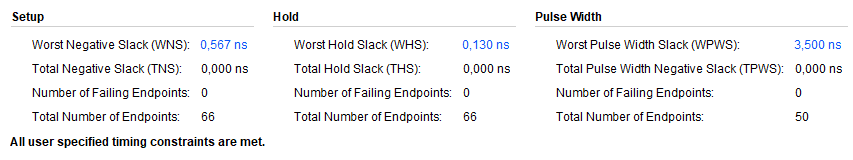
\includegraphics[width=1\textwidth]{img/Chapter5/ImplementationTiming.png}
    \caption{Timing Report}
    \label{fig:ITR}
\end{figure}

Even in this case there are \textbf{no negative slacks}, so a clock period of $8ns$ is fast enough. But in this case the \textbf{worst negative slack is worse} than before. This is due to the fact that the implementation allows to to obtain a more accurate estimate.

The \textbf{critical path} that cause this slack is the following:

\begin{figure}[H]
    \centering
    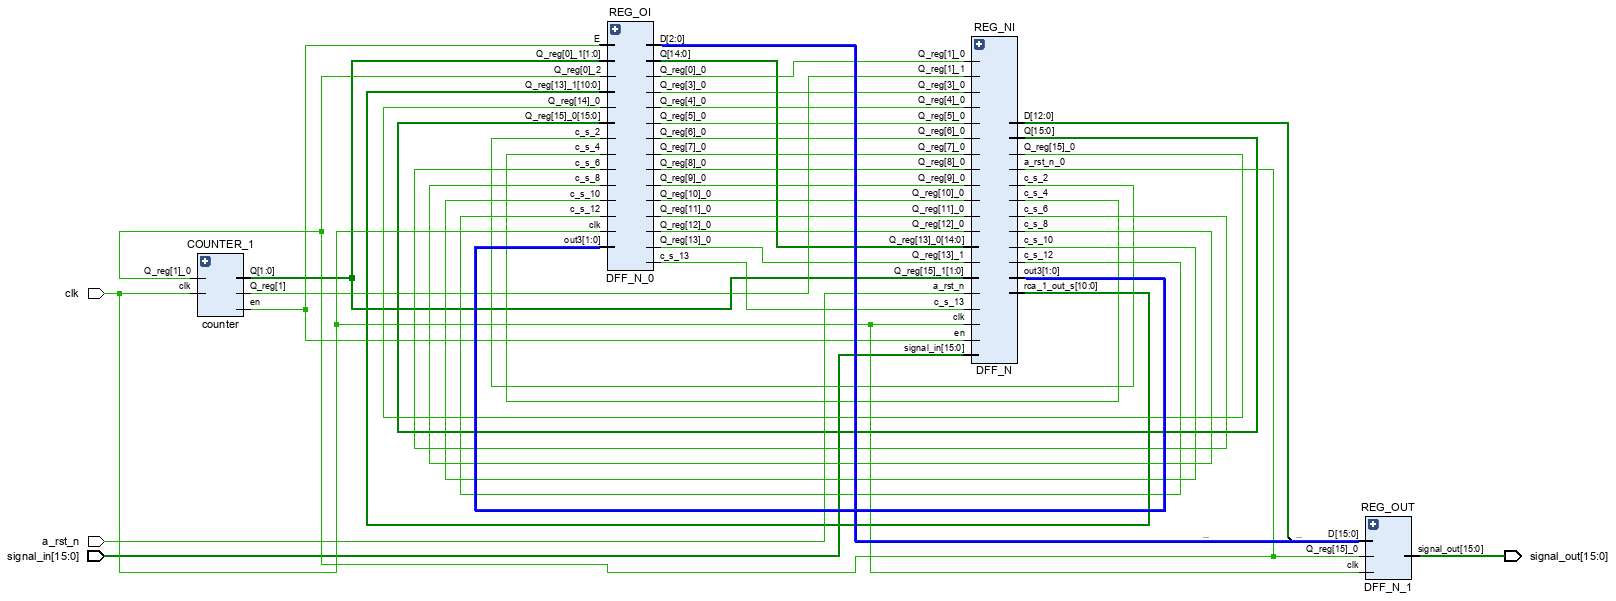
\includegraphics[width=1\textwidth]{img/Chapter5/ImplementationSetupCrit.png}
    \caption{Critical Path for Setup time}
    \label{fig:ICPS}
\end{figure}

\subsubsection{Utilization Analysis}

The \textbf{utilization report} obtained are as follows:

\begin{figure}[H]
    \centering
    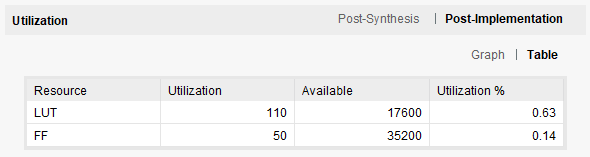
\includegraphics[width=0.6\textwidth]{img/Chapter5/ImplementationUtilization.png}
    \caption{Utilization Report}
    \label{fig:IU}
\end{figure}

Compared to the synthesis, the number of \textbf{Look Up Table} has increased to $110$, while the \textbf{Flip Flops} are the same.

\subsubsection{Power Consumption Analysis}

As regards power consumption, the results are the following:

\begin{figure}[H]
    \centering
    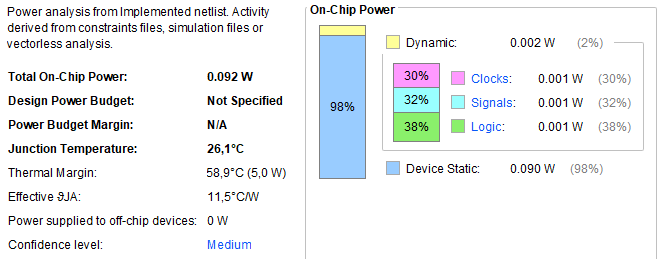
\includegraphics[width=1\textwidth]{img/Chapter5/ImplementationPower.png}
    \caption{Power Report}
    \label{fig:IPR}
\end{figure}

Compared to the synthesis, there are no changes.

\subsubsection{Warnings Analysis}

The Implementation's Warnings are the following:

\begin{figure}[H]
    \centering
    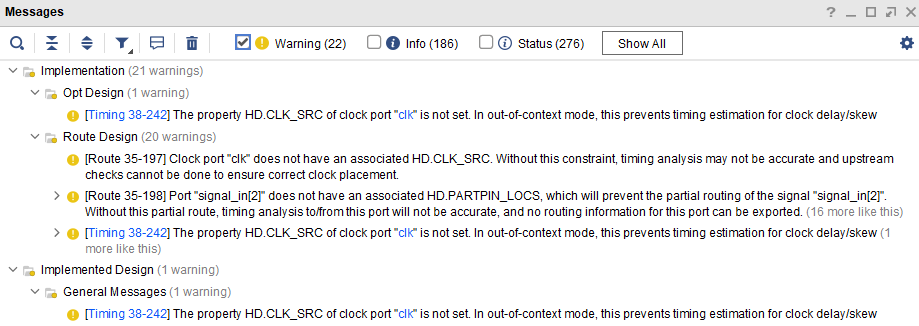
\includegraphics[width=1\textwidth]{img/Chapter5/ImplementationWarning.png}
    \caption{Implementation Warnings}
    \label{fig:IW}
\end{figure}

All of them are Vivado internal warnings, that can be ignored.